\documentclass{llncs}
\usepackage{amsmath}
\usepackage[show]{ed}
\usepackage{xspace}
\usepackage{paralist} % Used for the compactitem environment which makes bullet points with less space between them
%\usepackage{etoolbox}
\usepackage{enumitem}
\usepackage{eurosym}
\usepackage{graphicx}
\usepackage{wrapfig}
\def\stex{\texorpdfstring{\raisebox{-.5ex}S\kern-.5ex\TeX}{sTeX}\xspace}
\def\sTeX{\stex}
\usepackage{hyperref}

\def\degree{\ensuremath{^\circ}}
\newcommand{\sys}{\textsc{RPresentation}\xspace}

%----------------------------------------------------------------------------------------
%	TITLE SECTION
%----------------------------------------------------------------------------------------

\title{Relational Presentation Using Semantic Closeness\\Spatial Narrative for
  Mathematical Content}
\author{Naomi Pentrel, Michael Kohlhase}
\institute{Jacobs University Bremen}
%----------------------------------------------------------------------------------------
% Macros
%----------------------------------------------------------------------------------------

%----------------------------------------------------------------------------------------

\begin{document}
\maketitle

%----------------------------------------------------------------------------------------
%	ARTICLE CONTENTS
%----------------------------------------------------------------------------------------

 \begin{abstract}
Visualization of knowledge is important to foster learning. Especially so in Mathematics where students have to understand not just one topic at a time but also the related concepts. To optimize the visualization of information and its interdependencies, a way to present information without loosing context is necessary. The following research takes an existing annotated corpus and presents its contents in an interactive way that allows the audience to see the dependencies of the covered topics. This form of presenting knowledge enables users to interactively examine materials that are related to the topics the audience is interested in.

Taking the typical Mathematics lecture as an example, it is often the case that students have different backgrounds. Some might have learned linear algebra while other have not yet. Additionally, especially towards the end of the semester, students often have difficulties remembering earlier topics. When a new topic is introduced it would therefore be ideal to have a simple way to find dependencies and present students with an easy way to catch up.

The OMDoc (OpenMathematical Documents) format is a content markup scheme for mathematical documents. Using OMDoc, the proposed system can present different pieces of mathematical concepts in an interactive and connected way that allows students to learn the concepts the current topic depends on by taking a small detour through those topics, should they need to refresh their memories. Along these lines it examines if and how spatial narrative and semantic closeness can be combined to foster learning. This approach to presenting learning materials changes how we interact with course material which will allow students to learn better. Ultimately, this research is applicable to almost all areas in which knowledge needs to be transferred.
\end{abstract}

\section{Introduction \& Motivation}
\label{sec:introduction}

\begin{wrapfigure}{r}{0.36\textwidth}
\vspace{-2em}\centering
  \fbox{
    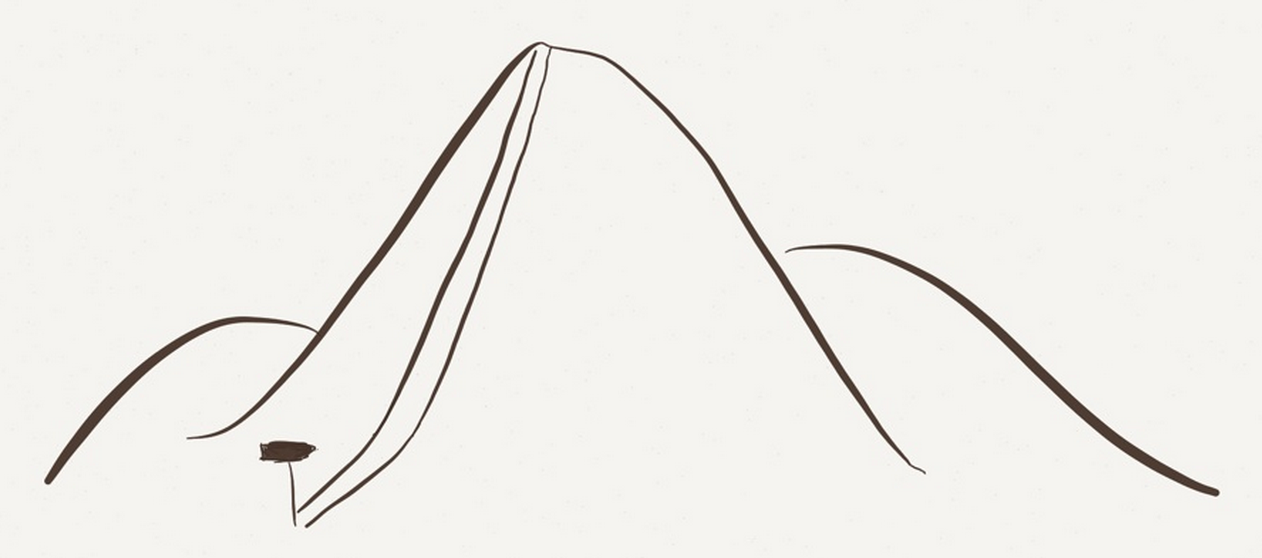
\includegraphics[width=0.36 \textwidth]{assets/final/straightMountain}}    \vspace{-20pt}
    \caption{Straight Learning Path}\label{fig:straight}
    \vspace{5pt}  
      \fbox{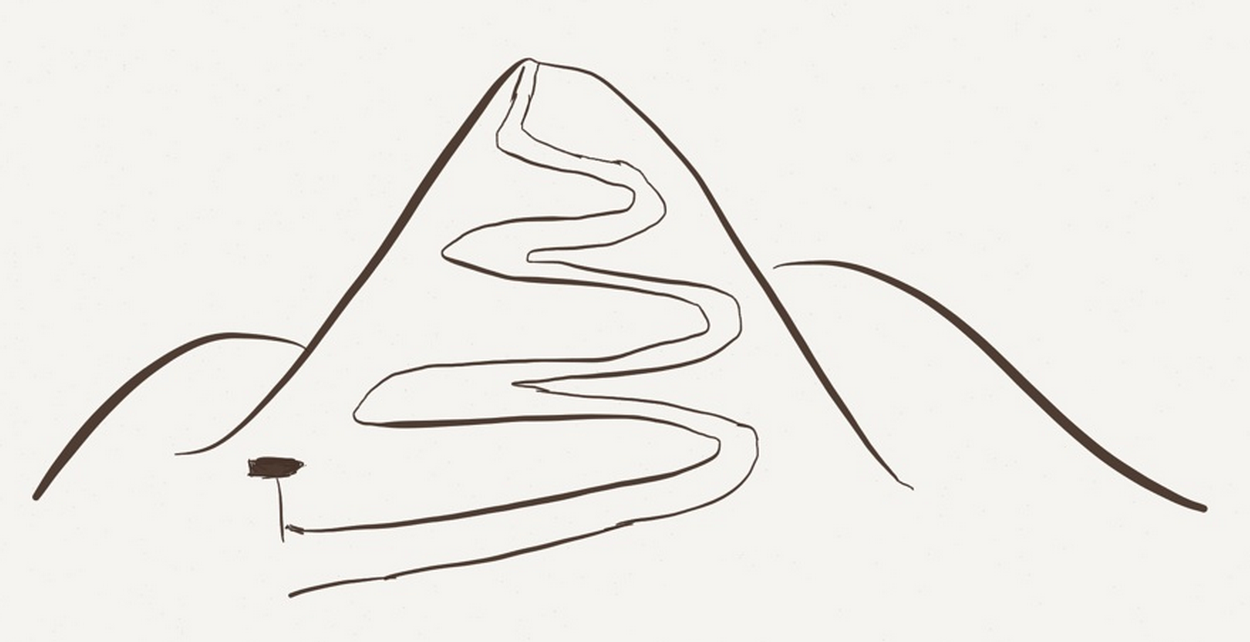
\includegraphics[width=0.37 \textwidth]{assets/final/curvyMountain}}
      \vspace{-20pt}
      \caption{Winding Learning Path}\label{fig:curvy}
      \vspace{-10pt}
\end{wrapfigure}

Learning new things is a bit like hiking up a mountain. If you have ever gone hiking, you know that it is hard to hike up a steep mountain directly as shown in \autoref{fig:straight}. Some people do it but most people will rather hike up as shown in \autoref{fig:curvy}. Both paths lead to the goal though. Within Mathematics classes, there is normally only one straight path and this has not changed in decades. With the advancement of technology, we are however able to change the way presentations and their narratives work. We can make it possible to link content that logically belongs together, in other words, content that is semantically close. Through the linking of content it becomes possible for a presenter to seamlessly lead an audience, not along a predetermined straight path, but rather along the path that allows the audience to take small detours and ultimately make the most out of the presentation.

\begin{wrapfigure}{l}{0.45\textwidth}\centering\vspace{-2em}
  \fbox{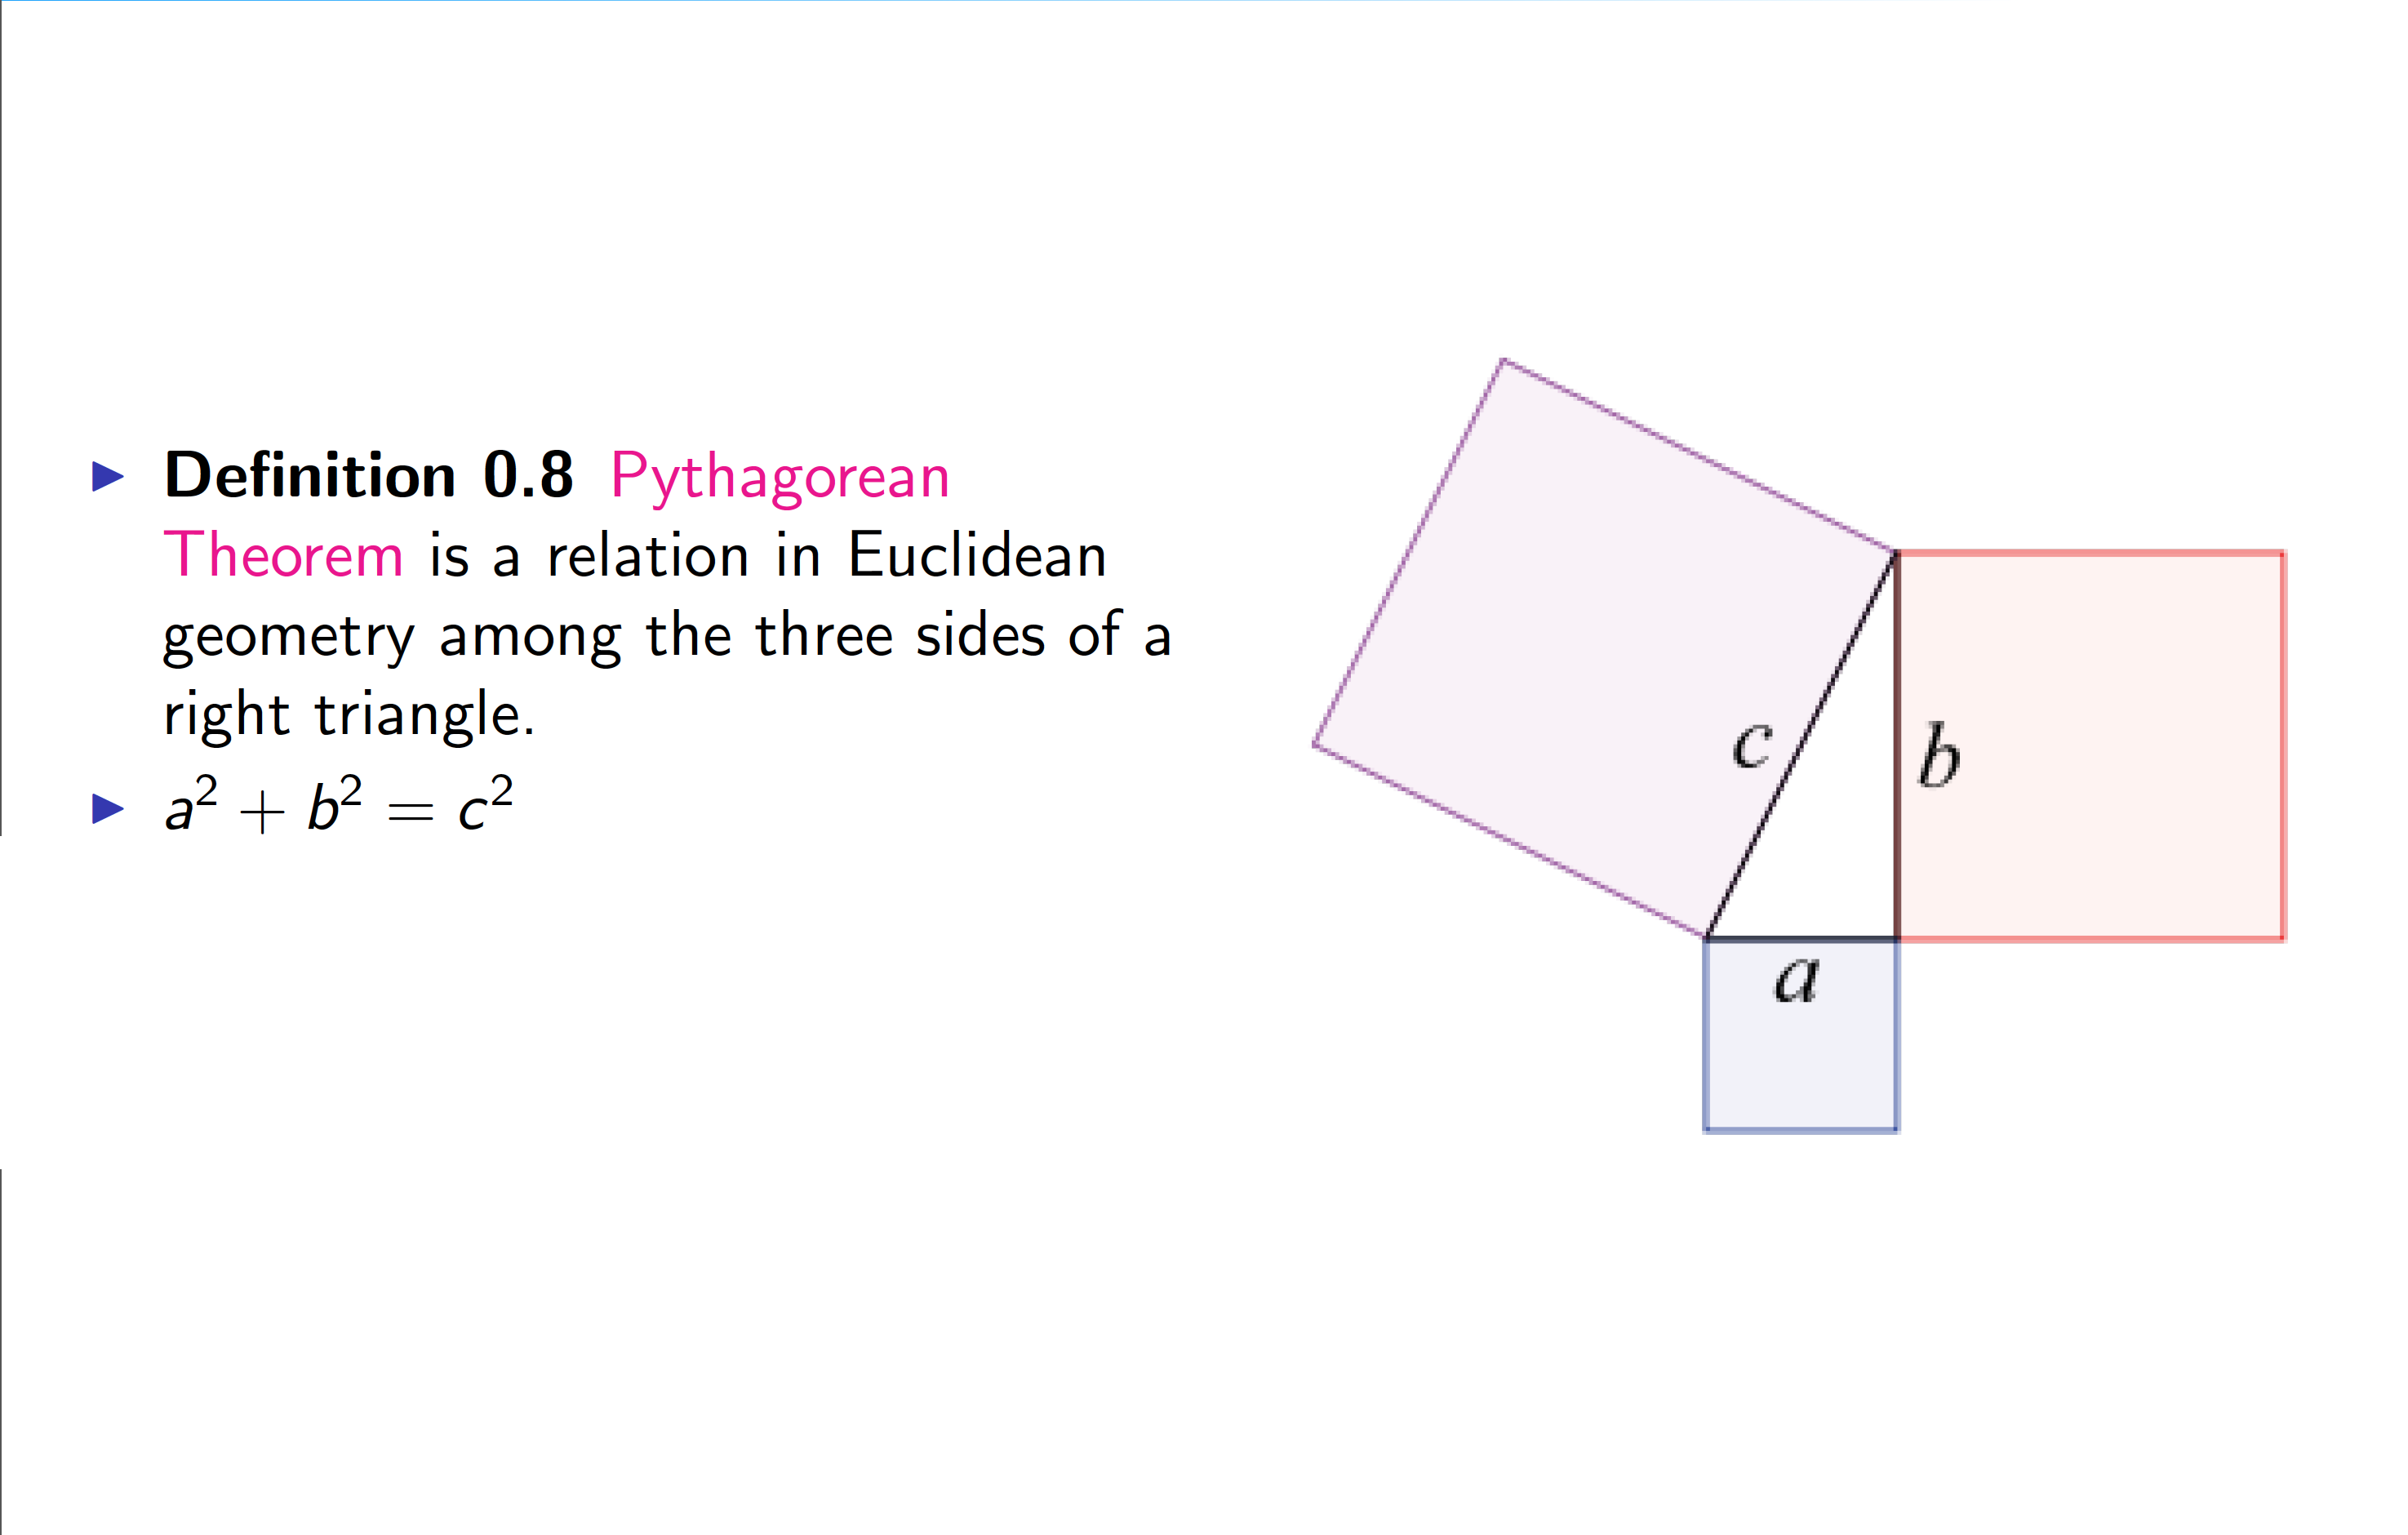
\includegraphics[width=0.43 \textwidth]{assets/final/slide_theorem}}\vspace{-.5em}
  \caption{Theorem Slide}\label{fig:slideP}
  \vspace{-15pt}
\end{wrapfigure}

Let us dive into a contrived story that will guide us throughout this research: Annie, a young student learning mathematics, is watching her teacher give a presentation on how to use the Pythagorean theorem (see \autoref{fig:slideP}). She is then given a triangle with sides a = 3 cm and b = 4 cm. Now she wants to use the theorem to calculate the length of side c. Annie already knows how to calculate the square of a number and thus calculates that $c^2 = 25 \implies c = 5$. However Annie made a mistake and did not know what a right triangle is. Her teacher tells her that the question was a trick question and that the answer is wrong because the triangle she calculated this for is not a right triangle. Now Annie has to try to find out what a right triangle is.

Annie's example shows the dependencies of different pieces of information, i.e. the Pythagorean theorem depends on knowledge of area calculation, lengths, squares, right angles, and angles. As Annie and many of us who have witnessed many presentations know, traditional slide-based presentations lack the connectivity and flexibility to allow us to directly look related topics up. However, especially in mathematics, students would benefit from the possibility to take detours through half-forgotten topics as topics are often closely linked and interdependent. By adding connectivity and flexibility, we would allow Annie to not just look up the prerequisite knowledge such as what right angles are but hopefully also to understand the Pythagorean theorem.

To achieve our goal to help Annie, we will set out to create a relational presentation system \sys to visually present information and its context which allows Annie to interact with the content and choose a path that matches her knowledge base. The visualization of the information will make use of spatial narrative to connect information in a logical way. Thus the final product will allow Annie to intuitively interact with the presentation to find the information she needs.

Along the way of helping Annie, we will explore the question of how to create a flexible presentation, which allows Annie to choose her own path to explore the context of a topic by browsing through related resources as needed. To create this presentation a tool for automatic contextual visualization of information will be introduced. Through the usage of both spatial narrative and semantic closeness of information it will connect information logically. The end product will be a presentations which allow Annie to choose her own path by interacting with the presentation to seamlessly explore related topics and brush up on half-forgotten topics like right angles. There are many stories such as Annie's in real life and it is therefore important to provide information with its context to facilitate learning and knowledge transfer as a whole so that each of us can choose a learning path that allows us to reach the goal, whether it be by following a straight or a curvy path.

\section{Towards a More Effective Presentation Format}
\label{sec:TowardsAMoreEffectivePresentationFormat}

We will now commence the journey towards building a more effective presentation format to improve knowledge transfer in Mathematics by allowing flexibility in presentations. In the following we will assume the reader is familiar with OMDoc \cite{Kohlhase:OMDoc1.2} and with the open-source presentation framework \textit{impress.js} \cite{JSImpress:npentrel14} which will be used to create the final presentation in the form of an interconnected network of information that tells a visual story based on semantic closeness to facilitate the transfer of knowledge. To create these presentations automatically, the tool \sys \cite{npentrel:npentrel15} was created. 

\begin{wrapfigure}{l}{.55\textwidth}\centering\vspace{-2em}
  \fbox{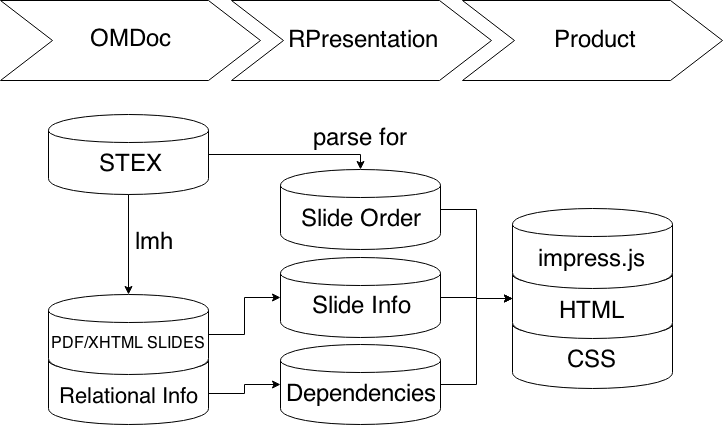
\includegraphics[width=0.55\textwidth]{assets/final/Architecture}} 
  \vspace{-1em}
  \caption{Architecture Diagram}\label{fig:architecture}\vspace{-1em}
\end{wrapfigure}

With the OMDoc framework and its tools it is possible to write down course notes or other documents in \textbf{S}emantically enhanced \TeX / \LaTeX\ (\stex). The Local MathHub Tool (lmh) uses these to create, among other things, PDF slides, XHTML slides, and relational information. To help Annie, let us use a document that explains the Pythagorean theorem and related topics. The files that lmh creates, along with the \stex -files will be used as input in the next steps. For the implementation of  \sys Java was used.

\sys itself operates in five main steps:
\begin{enumerate}[topsep=0pt,itemsep=-1ex,partopsep=1ex,parsep=1ex]
\item Get user input for the locations and names of folders.
\item Parse \sTeX to retrieve the order of slides.
\item Extract dependencies from relational info.
\item Extract necessary XHTML or PNG parts for slides.
\item Create presentation.
\end{enumerate}
\vspace{5pt}

After asking the user for the location and names of the folders we want to work on, \sys can parse the provided \stex files in a recursive fashion to retrieve the slide order. It does this by starting with a given top level file which includes other files via \textit{mhinputref}s.

In the next step the relational information is parsed and put into a hashtable. The keys are the slides which link to an array of dependent slides. The order of the slides and their dependencies are then combined to an information graph which we use to create a relational presentation out of the annotated document using the slide info. This slide information is created by either parsing the XHTML and directly copying the needed parts into the final presentation or by transforming the PDF into PNGs that are then included in the final presentation.

For including the XHTML or the PNGs we use self-created boilerplate code, in which only some coordinates and the XHTML or the PNGs for the slide are added. The details of this process will be explained in subsection \ref{sec:narrativePaths}, \ref{sec:orderedInfoGraphs}, and \ref{sec:levels}. To complement the HTML, a CSS stylesheet is added which adds the some design elements. The design of the template is based on a presentation by S. Wolf \cite{Wolf:npentrel15}. To bring the presentation to life the library impress.js is used because it makes it simple to reuse the XHTML code that was automatically generated by lmh. An important additional reason for the choice of impress.js \cite{JSImpress:npentrel14} is that it enables us to use spatial narrative.

\subsection{Status of Information within the (Dis)Course}
\label{sec:infostatus}
In linguistics the concept of information packaging \cite{CambridgeGrammar:npentrel14} is well known and widely discussed. Within the study of \textit{information structure}, one discriminates between \textit{familiar/ old} and \textit{unfamiliar/ new} information. \textit{Familiar/ old} information is shared by speaker and addressee, i.e. it is in the intersection of knowledge of student and teacher. \textit{New/ unfamiliar} information is not in the shared knowledge base or the content commons \cite{CNX:whitepaper}. In addition, one distinguishes information that is old or new with respect to the discourse or with respect to the addressee.

\begin{center}
\textit{"My sister went to the circus the other day; \underline{she} said \underline{it} was brilliant."}
\end{center}

In this example in the first part of the sentence, \textit{discourse-new} information pertaining to my sister and to a circus is introduced. In the second part, the underlined parts are considered \textit{discourse-old} since they have already been introduced. These terms are coined to refer to the accessibility of the information to participants of the discourse \cite{Newness:npentrel14}. The accessibility depends on the relative \textit{newness}, i.e. recency of mention, of this information.

These concepts can be adapted to the situation of teaching mathematics or computer science to students in a class. In general we will call the information that the speaker is passing on to the addressees/students \textit{course-new}. Since we are in a classroom setting, the \textit{course-new} information will generally depend on information that is \textit{course-old}. We will additionally introduce a third modus for information called \textit{course-ancient}. This covers the situation where the addressee has difficulties following the speaker since the \textit{course-new} information depends on \textit{course-old} information that might be 'too old' to be easily remembered, i.e. \textit{course-ancient}.

Going back to the example of Annie, the information about the Pythagorean theorem that the teacher is just introducing would be considered \textit{course-new}. The information about the right angle which Annie cannot access anymore since she was taught about this too long ago is \textit{course-ancient}. The information about squares which Annie still remembers is \textit{course-old}. Through the semantic closeness that OMDoc provides, we will be able to determine the status of information within the (dis)course.

\subsection{Narrative Paths}
\label{sec:narrativePaths}

The information that OMDoc provides us with could also be simply visualized as a tree of information. However, this would not be very engaging and it would be hard for a person to process. Similarly, traditional slide-based presentations do not provide a very engaging or interactive form of presenting information. Therefore we will focus on using spatial narrative to make presentations more engaging and enhance knowledge transfer. 

One opportunity to employ spatial narrative is to place content which is inherently related visually close together since this conveys the meaning that these objects belong together. In \textit{A mathematical approach to ontology authoring and documentation} \cite{LK:MathOntoAuthDoc09}, it is stated that "documents consist of narrative and content layers". In our case, the content layers are the mathematical objects, i.e. the statements or theories. Narrative layers refer to the order in which the mathematical objects from content layers are presented.

\begin{wrapfigure}l{.65\textwidth}\vspace{-2em}
  \fbox{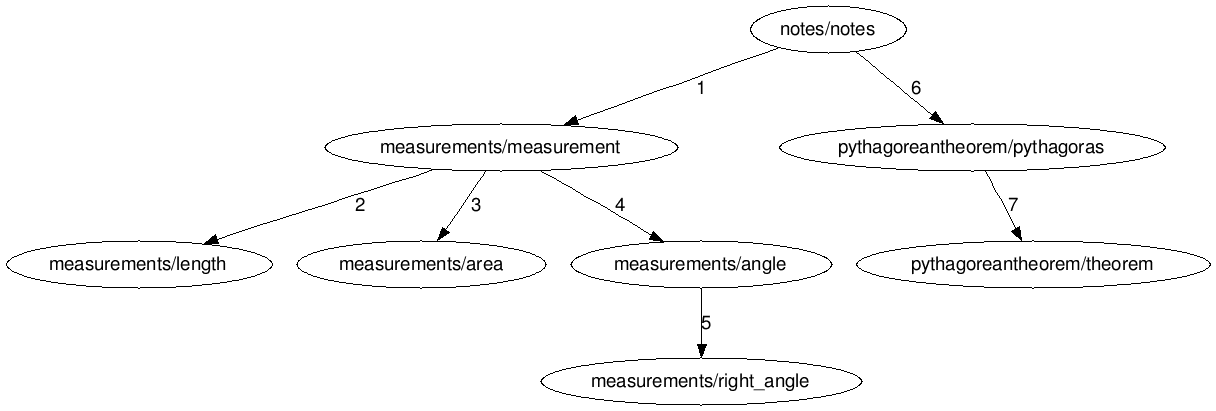
\includegraphics[width=0.65\textwidth]{assets/final/inclusionGraphPythagorean}} 
  \caption{Inclusion Graph for the Pythagorean Theorem}\label{fig:inclusionGraph}
\end{wrapfigure}

In our system, the \stex files are parsed using a Depth First Search algorithm to retrieve the narrative the writer intended to use. For the explanation of the Pytha\-go\-rean theorem this can be seen in \autoref{fig:inclusionGraph}. We will refer to this intended narrative layer as the \textit{primary narrative path} which we follow from slide to slide on our path to the end of the presentation. To create this primary narrative path we need to add several slides with increasing x-coordinates as portrayed in \autoref{fig:primaryNarrativePath}.

\begin{wrapfigure}{c}{\textwidth}\centering\vspace{-2em}
  \fbox{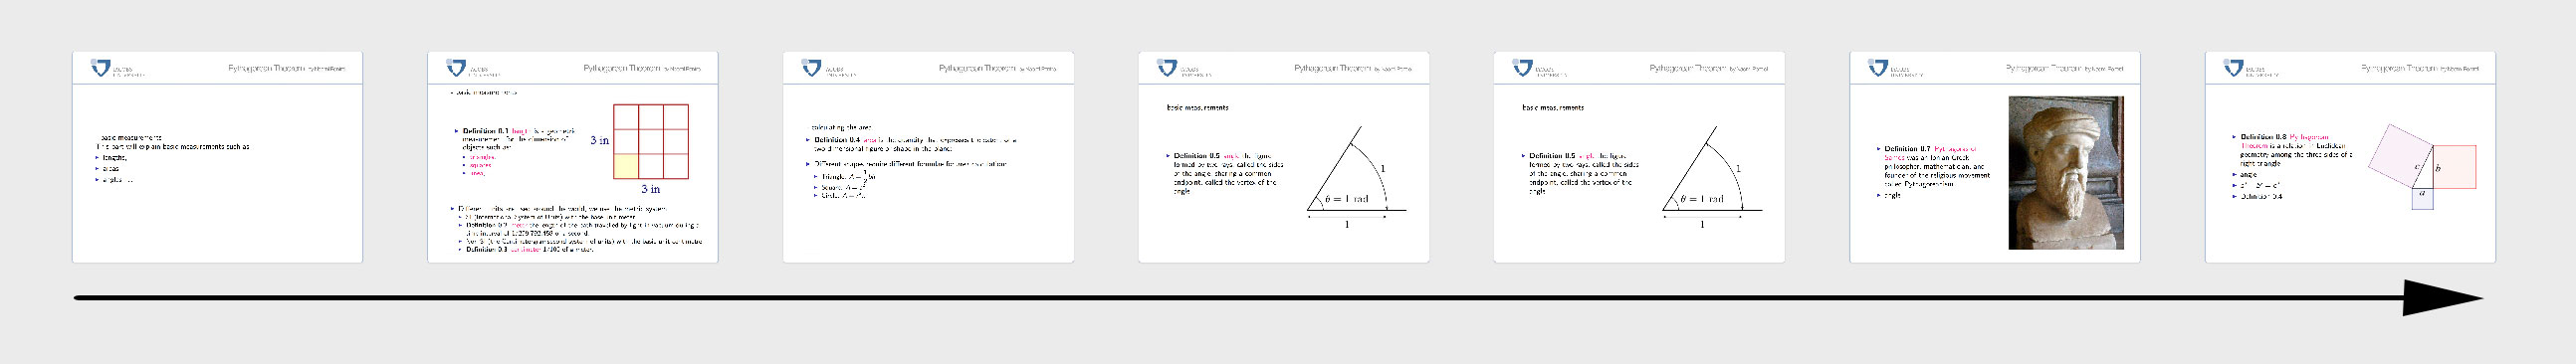
\includegraphics[width=0.97\textwidth]{assets/final/primaryNarrativePath2}}
  \vspace{-1em}
  \caption{Primary Narrative Path}\label{fig:primaryNarrativePath}
  \vspace{-1em}
\end{wrapfigure}
The primary narrative path, formed by a horizontal stream of slides, is the traditional
path a presenter normally uses when preparing a PowerPoint presentation. Thus it contains
also temporal information which is illustrated by the arrow in
\autoref{fig:primaryNarrativePath}. This temporal information is what we extracted from
the \stex files as the order in which the slides (or the information on the slides) should
appear.

Temporal information is also used to create narrative paths for subsections of the whole presentation that only explain one topic. These narrative paths are similar to short guided tours in that they aim to explain one topic but they are different in that they just reuse slides that have already occurred. Going back to our example of Annie, an example of a subsection would be the information concerning angles. In essence, the \textit{intended narrative path} contains multiple \textit{narrative paths} of its own which occur on different levels as explained in \autoref{sec:levels}.

\subsection{Ordered Information Graphs}
\label{sec:orderedInfoGraphs}

As described in \autoref{sec:TowardsAMoreEffectivePresentationFormat}, lmh outputs information about dependencies of topics. \sys parses this relational data and retrieves the dependencies of the topics which are visualized for Annie's example in \autoref{fig:depGraphPythagoreanFull}. Dependencies give us the \textit{course-ancient} information, as dependencies intuitively link to information obtained longer ago.

\begin{figure}[ht]\vspace{-1em}
  \fbox{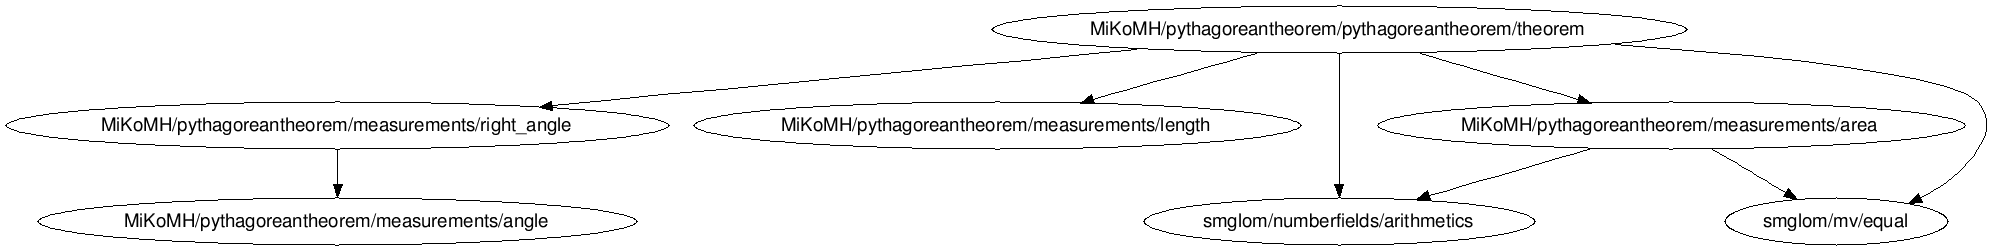
\includegraphics[width=0.97\textwidth]{assets/final/dependencyGraphPythTheo2}} 
  \vspace{-.5em}
  \caption{Dependency Graph}\label{fig:depGraphPythagoreanFull}
\end{figure}

\begin{wrapfigure}r{.67\textwidth}\vspace{-2em}
  \fbox{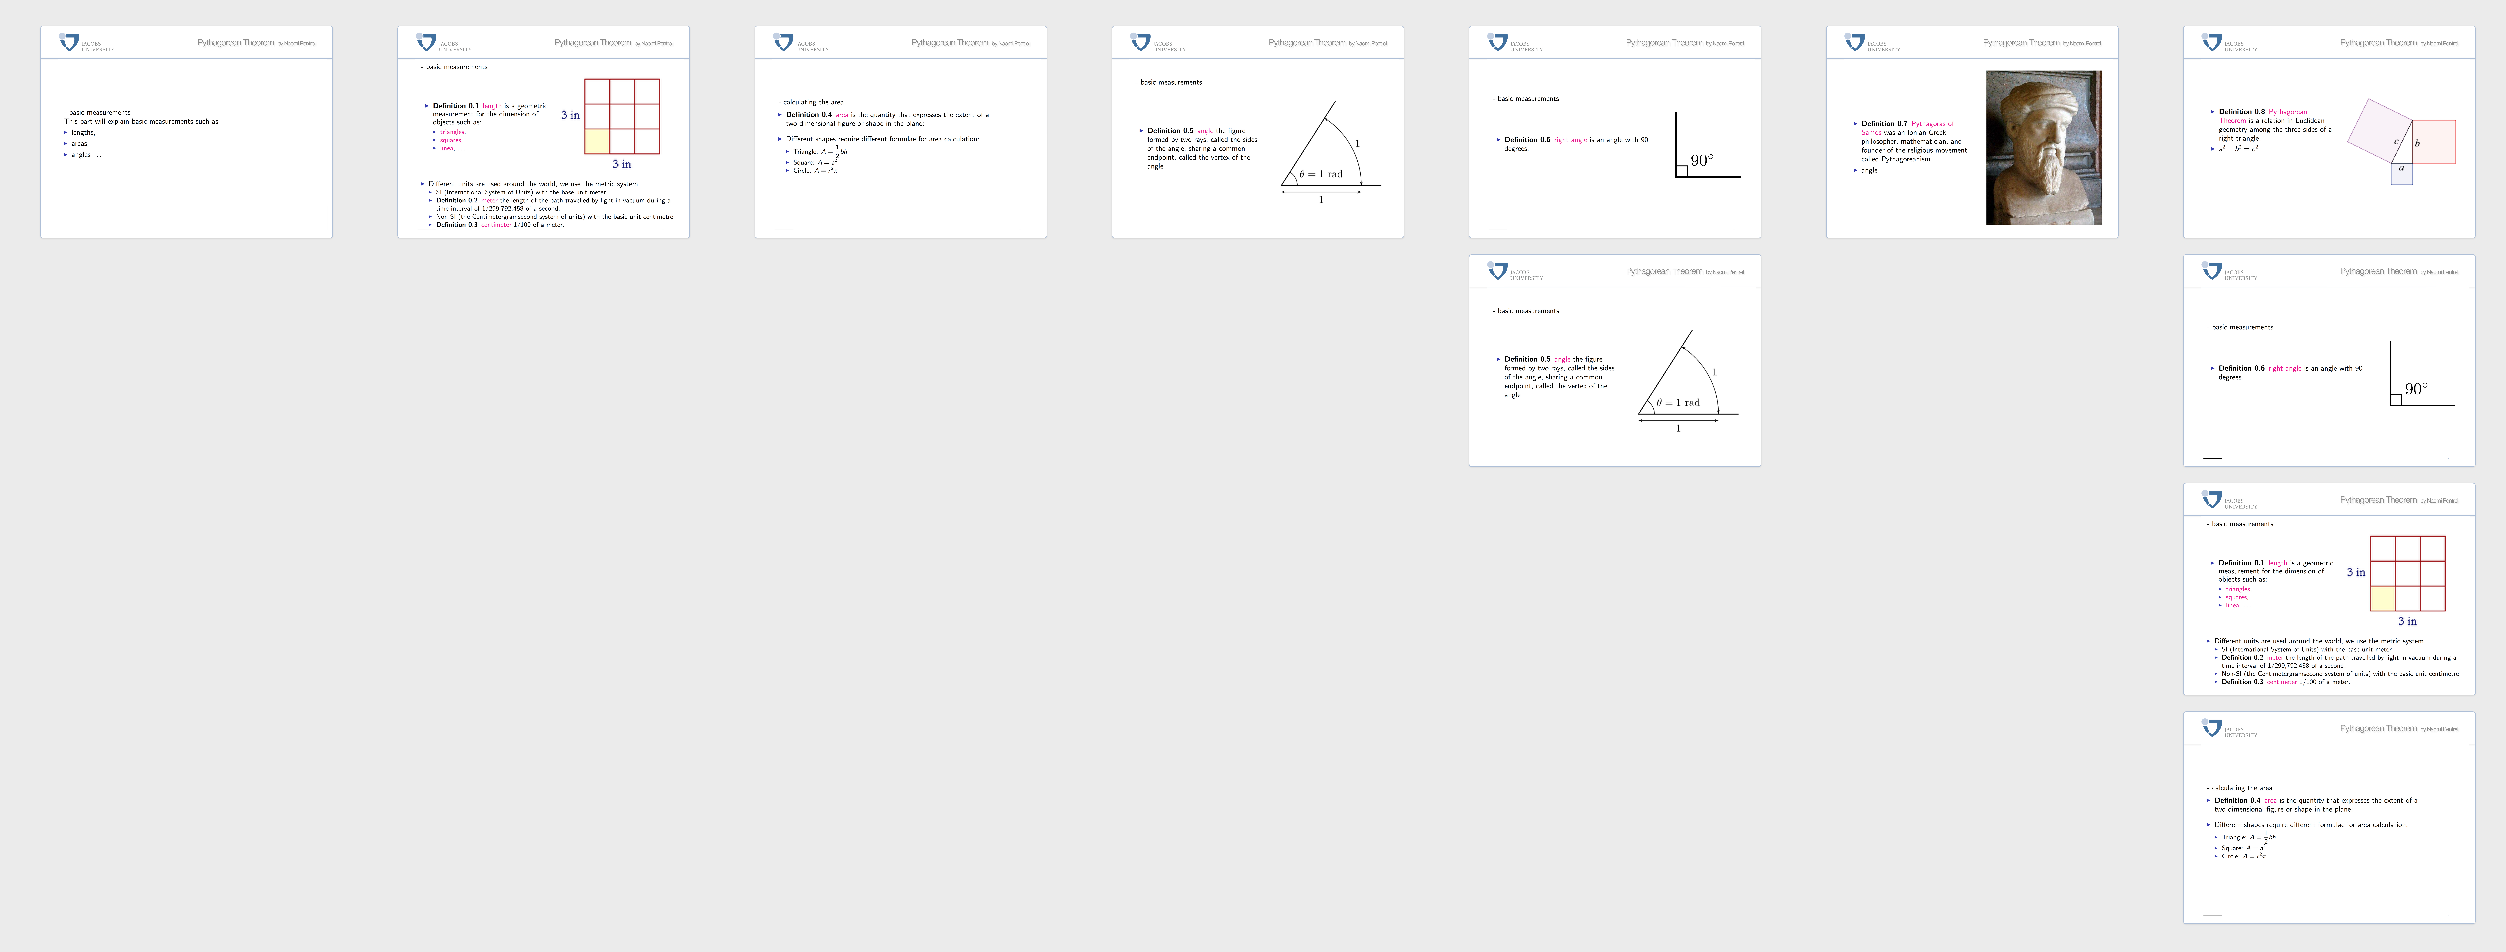
\includegraphics[width=0.67\textwidth]{assets/final/fullPresentation2}} 
  \vspace{-1em}
  \caption{Visualization of Dependencies}\label{fig:visualDependency}
  \vspace{-1em}
\end{wrapfigure}
With the data about the order and the dependencies of information within the paper, we now
have an ordered information graph out of which we can build a first presentation that
Annie can interact with to learn about the Pytha\-go\-rean theorem. \sys creates this
presentation incrementally. As outlined in \autoref{sec:narrativePaths} and illustrated in
\autoref{fig:primaryNarrativePath}, \sys creates the primary narrative path from the order
of the slides. After adding each slide it checks whether there is \textit{course-ancient}
information, i.e. whether there are dependencies, for that slide. If there are
dependencies those are added below the slide itself (see
\autoref{fig:visualDependency}).\footnote{library impress.js was adapted to support the
  choosing of different paths by pressing the right or down key
  \cite{npentrel:npentrel15}.}


\subsection{Levels}
\label{sec:levels}

\begin{wrapfigure}r{.6\textwidth}\vspace{-2em}
  \fbox{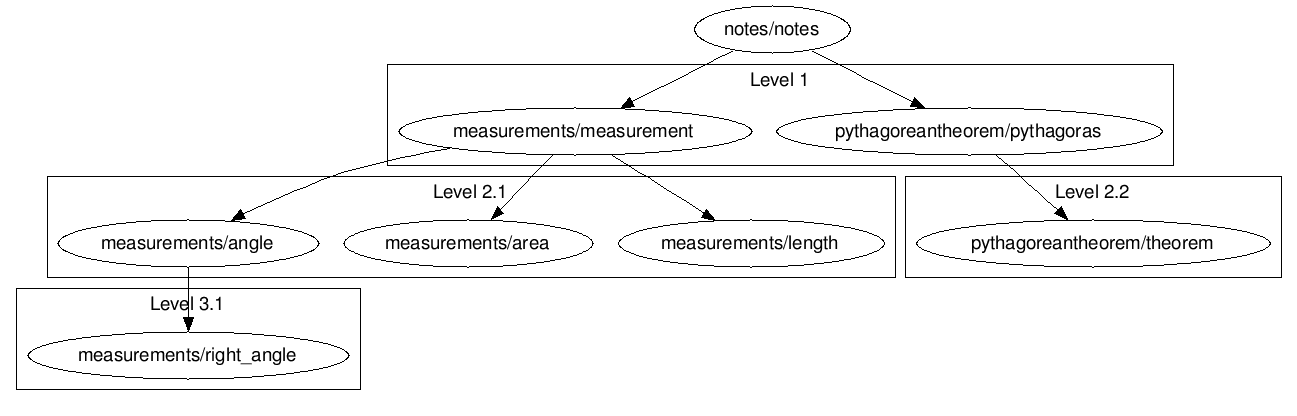
\includegraphics[width=0.6\textwidth]{assets/final/levels}} 
  \vspace{-1em}
  \caption{Inclusion Graph with Levels}\label{fig:levelsGraph}
\vspace{-1em}
\end{wrapfigure}
When writing a document or course notes in \stex, the creator general writes a top-level
file such as \textit{notes.tex} from where other \TeX\ files are included. These included
files again include further \TeX\ files etc.. Thus we are automatically provided with
levels that we can use for splicing our primary narrative path into smaller narrative
paths. In essence, on any level the order of information in that topic is a narrative path
itself. Expressed in mathematical notation a level within a directed graph
$G = \langle V, E \rangle $, with $V$ being a set of nodes and $E = V \times V$ being the
set of directed edges, is the set
$L_w = \lbrace v \vert \langle w, v \rangle \in E \rbrace$. From these levels we can infer
the status of the information. We already know that a dependent piece of information
infers that it is \textit{course-ancient} information. Anything that is on the same level
or in the sublevels thereof is considered to be \textit{course-old} information.

\begin{wrapfigure}{l}{0.43\textwidth}\vspace{-2em}
  \fbox{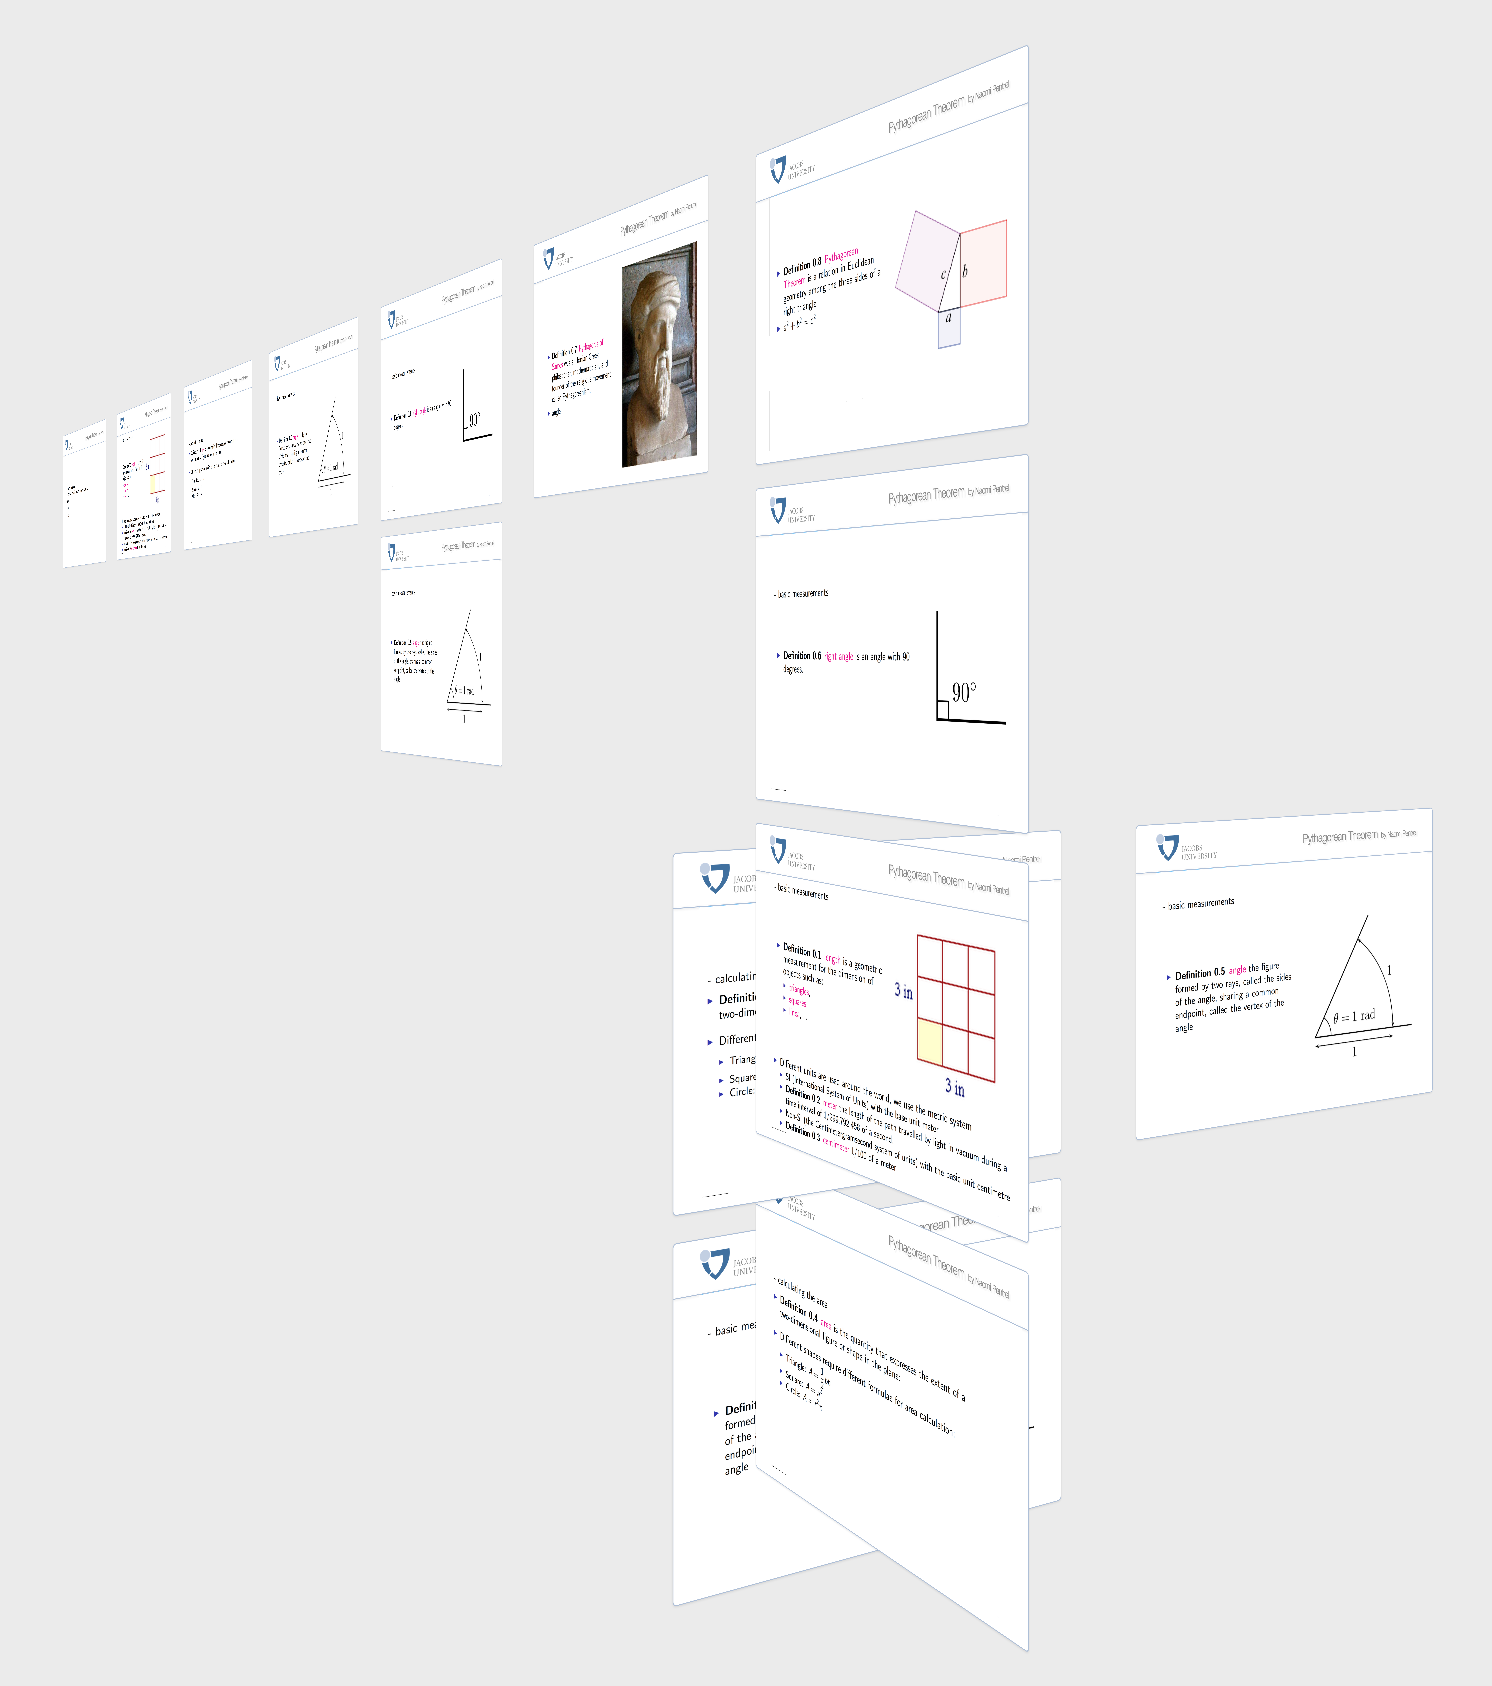
\includegraphics[width=0.4\textwidth]{assets/final/60degree}} 
  \vspace{-.5em}
  \caption[Caption for LOF]{Visualization\footnotemark of Dependencies and Levels at
    60\degree}
  \label{fig:visualDependencyDegree}
\vspace{-1em}
\end{wrapfigure}
If Annie, while browsing through the different dependencies, realizes that she needs to
refresh her memory or learn more about any of the dependent information she can enter the
respective level. The presentation will then continue on that level and show all the
slides from that topic in the correct order. Once Annie has gone through this short
excursion, she can return to the initial slide and resume the primary narrative path. By
adding a way to explore these other levels, the presentation adds more context and allows
Annie to understand the subject on a deeper level. These modular excursions are included
in the presentation in 3D by making use of CSS3-transitions. Thus when the user enters an
excursion a 90\degree\ rotation around the y-axis occurs and the user can now follow that
story line (see \autoref{fig:visualDependencyDegree}).

\footnotetext{The overlapping slides do not interfere as they are at a 90\degree\
  angle. Therefore when seeing one slide, the other slide will be visible only from the
  side. Since a slide is very thin this makes it invisible.}

\subsection{The Relational Presentation}
\label{sec:RelationalPresentations}

Combining the information about narrative paths, dependencies, and levels, we derived an ordered information graph out of which we have built a presentation that Annie can interact with to learn about the Pythagorean theorem. In this section we will examine the structure of the created presentation.

To begin with, let us examine the choice of layout. The goal of this presentation is to have all the information the Pythagorean theorem depends on easily accessible so that Annie can access \textit{course-ancient} information easily. The added expressiveness that impress.js offers allowed us to have this in a very structured format while focusing on visualizing relations between content with movement and closeness. This also serves to keep the resulting presentation simple and easily usable.

While focusing on closeness and movement, it creates meaningful visual relations and semantic movements. The relations between the content, such as it being the next slide in the narrative or it being a dependency are shown through the closeness and the placement of the slide as well as the movements that come with it. The following movements exist:
\begin{inparaenum}[\em a\rm)]
\item movement along the x-axis,
\item movement along the y-axis, and
\item rotations.
\end{enumerate}

The movement along the x-axis has a mostly temporal semantics associated with it. Going to the left is connected with going backwards in the narrative, whereas going to the right is associated with going forwards in the narrative. Apart from going forwards and backwards, we can also move along the y-axis. Moving down intuitively means that we dig deeper into a topic and go to the roots of a problem, whereas moving back up means we will be on a higher level.

The most interesting movement is the rotations which aim to give the viewer the feeling of
entering a topic and a different storyline. Thus entering a different topic comes with a
change of perspective which is underlined by the 3D transformation that the user
sees. Overall, these movements add expressiveness to the relations and allow for intuitive
interaction with the presentation. \footnote{To see the presentation in action visit:
  \href{http://npentrel.github.io/pythagoreantheorem.html\#/overview}{http://npentrel.github.io/pythagoreantheorem.html\#/overview}.}

One might think that this is similar to a PowerPoint presentation, since PowerPoint offers
similar animations to switch slides. The important addition is more obvious when regarding
the presentation from a bird's eye perspective by looking at the overview in
\autoref{fig:visualDependency} or \autoref{fig:visualDependencyDegree}. The value in these
presentations is that dependencies become identifiable. More importantly this means that
for Annie, dependencies become accessible and allow her to go on small guided tours or
small excursions into \textit{course-ancient} topics giving her the flexibility to choose
her own path while going through the presentation.

\section{Conclusion}
\label{sec:conclusion}

We set out to help Annie understand the Pythagorean theorem. Her problem was that she did not know about some of the dependent information, i.e. right angles, and since there was no easy way to access this information she could not understand the topic fully. To help her, we created a system \sys that parses the documents that the instructor wrote and created a relational presentation out of it.

This relational presentation combines spatial narrative with information about the relations between different pieces of information into a visual information graph. In doing so it creates presentations that use meaningful visual connections between pieces of information to allow for intuitive interaction with the presentation. This allows Annie to choose her own path while going through the presentation and seamlessly looking up related information.

The benefits are not just for Annie when she is going through the presentation on her own though, Annie's teacher now has a tool that allows him to use his normal lecture material in a more interactive way. Thus when the teacher realizes that the students need to revise previous material, the teacher can seamlessly go to that material and provide them with a good learning experience. These digressions are the added value that allow flexibility in these new presentation and transform the traditional presentations from linear presentations to relational presentations. Overall this facilitates knowledge transfer and allows for a more engaging and interactive education.

Linking learning materials is useful for knowledge transfer and especially mathematics is a field that could profit from guided tours through topics as a way of learning topics according to users' individual knowledge bases. In future, I believe that this research could be adopted in more fields, transforming education into something that allows individuals to learn the way that is best for them. In the introduction, I introduced the metaphor of hiking up a mountain which can be done in different ways. The type of presentations this research built allows for a lot of different paths to reaching a learning goal. The flexibility that comes with these presentations is undoubtedly preferable to traditional presentations as it offers clear benefits in allowing to effortlessly change the path of the presentation at any point.

To conclude, I leave the reader to ponder how much education would change if we could allow individuals to learn at their own pace following their own path and easily learning course-ancient information in guided tours. \sys definitely helped Annie and I strongly believe that the mentioned benefits would benefit all of us, whether in the role of the presenter or in the role of the viewer.


\bibliography{kwarc}
\bibliographystyle{alpha}
\end{document}

%%% Local Variables:
%%% mode: latex
%%% TeX-master: t
%%% End:
